\documentclass{article}
\usepackage{graphicx} % Required for inserting images
\usepackage[utf8]{inputenc}
\usepackage[T1]{fontenc} 
\usepackage[polish]{babel}
\usepackage{hyperref}
\usepackage{graphicx}

\title{\textbf{Specyfikacja implementacyjna programu dzielącego graf}}
\author{Adam Domański, Oliwier Osiński}
\date{28.04.2025}

\begin{document}
\maketitle

\section*{Struktura plików}
Opisywany program składa się z następujących katalogów i plików:
\begin{itemize}
    \item Makefile - plik wykonywalny kompilujący i uruchamiający różne testowe scenariusze programu;
    \item bin - katalog zawierający skompilowany program o nazwie "graf";
    \item include - katalog zawierający pliki nagłówkowe;
    \item src - katalog zawierający pliki źródłowe c;
    \item tests - katalog zawierający testowe pliki wejściowe opisujące grafy
\end{itemize}

\section*{Argumenty wywołania}
Do poprawnego uruchomienia programu niezbędne jest podanie jednego obowiązkowego argumentu. Opcjonalnie można dodać dwa dodatkowe argumenty zmieniające parametry programu.
\begin{enumerate}
    \item \textbf{plik.in} - ścieżka do pliku, w którym zapisany jest graf przeznaczony do podziału.\\\\
    W przypadku, gdy podany plik nie istnieje, program zróci błąd o treści: Blad: Nie udalo sie otworzyc pliku wejsciowego o podanej sciezkce. Przerywam dzialanie.\ i zakończy działanie.\\\\
    Natomiast, gdy dane przedstawiające graf są niepoprawne, program zwróci błąd o treści: "Blad: Dane w pliku przedstawiajace graf sa niepoprawne. Przerywam dzialanie."\ i zakończy działanie.
    
    \item \textbf{N} (opcjonalny) -  dodatnia liczba całkowita podzieleń grafu na podgrafy, której wartość domyślna wynosi \textbf{1}.\\\\
    W przypadku, gdy nie poda się wartości liczbowej, program zwróci błąd o treści: "Blad: Liczba podzieleń grafu została niepoprawnie zdefiniowana. Przerywam działanie."\ i zakończy działanie.\\\\
    Natomiast, gdy podana liczba, będzie niedodatnie lub zmiennoprzecinkowa, to program zwróci błąd o treści: "Blad: Liczba podzieleń grafu musi być większa bądź równa 1. Przerywam działanie."\ i zakończy działanie.

    \item \textbf{M} (opcjonalny) - nie ujemna liczba całkowita nie przekraczająca wartości 100, liczba przedstawia graniczną wartość procentową, pod którą musi się zmieścić różnica wierzchołków podzielonych podgrafów, jej domyślna wartość wynosi \textbf{10}.\\\\
    W przypadku, gdy nie poda się wartości liczbowej, program zwróci błąd o treści: "Blad: Liczba marginesu różnicy procentowej została niepoprawnie zdefiniowana. Przerywam działanie."\ i zakończy działanie.\\\\
    Natomiast, gdy podana liczba, będzie ujemna lub zmiennoprzecinkowa, to program zwróci błąd o treści: "Blad: Liczba marginesu różnicy procentowej między wierzchołkami powstałych grafów musi znajdować się w przedziale [0-100]. Przerywam działanie."\ i zakończy działanie.
\end{enumerate}


Przykłady użycia argumentów podczas wywoływania programu znajdują się w sekcji \textbf{Uruchomienie programu}.

\section*{Flagi}
Program przyjmuje następujące flagi:
\begin{itemize}
    \item \textbf{-h} - flaga wyświetlająca informacje o argumentach programu oraz dostępne flagi wraz z ich opisami.
    \item \textbf{-o plik.out} - flaga przyjmująca jako argument ścieżkę do pliku, do którego ma zostać zapisany wynik końcowy programu. Domyślna wartość argumentu flagi to \textbf{"wynik.txt"}.

    \item \textbf{-b} - flaga zmienia tryb wyświetlania wyniku z domyślnie tekstowego na binarny.

    \item \textbf{-t} - flaga sprawiająca, że wynik końcowy programu zostanie wypisany w terminalu. Można łączyć z flagą -b, wtedy w terminalu zostanie wyświetlony wynik binarny.
\end{itemize}

Przykłady użycia flag podczas wywoływania programu znajdują się w sekcji \textbf{Uruchomienie programu}.

\section*{Uruchomienie programu}
Do kompilacji programu należy użyć komendy \textbf{make} w terminalu lub od razu wybrać wcześniej przygotowany scenariusz testowy, wpisując \textbf{make \{nazwa\_testu\}} o których więcej w sekcji \textbf{Testy}.
\\

Aby uruchomić program należy w teminalu wywołać plik wykonywalny znajdujący się w katalogu bin: \textbf{/bin/graf}, a następnie podać odpowiednie argumenty, o których mowa była w sekcjach \textbf{Argumenty wywołania} oraz \textbf{Flagi}.\\

Przykład wywołania programu wczytującego graf z pliku /tests/graf.csrrg, wypisującego wynik w trybie tekstowym w terminalu oraz do pliku podzial.txt:
\textbf{./bin/graf /tests/graf.csrrg 2 20 -o podzial.txt -t}\\

Przykład wywołania programu wczytującego graf z pliku /tests/graf2.csrrg, wypisującego wynik w trybie binarnym w terminalu oraz do wynik.txt:\\
\textbf{./bin/graf /tests/graf2.csrrg -t -b}

\section*{Format wyjściowy}
Program zawsze zapisuje końcowy wynik w pliku, który został podany w odpowiedniej fladze podczas wywoływania (domyślnie "wynik.txt").\\

Na wynik końcowy w trybie tekstowym (domyślny) składa się:
\begin{itemize}
    \item Liczba udanych podziałów grafu w pierwszej linijce.

    \item Następnie graf w takim samym formacie co w pliku wejściowym.
\end{itemize}

W przypadku trybu binarnego, podawany jest jedynie sam graf. Sposób zapisania grafu w postaci binarnej przedstawia sekcja \textbf{Plik binarny}.

\section*{Plik binarny}
Sposób zapisania grafu do pliku binarnego, odbywa się poprzez zapisanie każdego znaku, z oryginalnego formatu zapisu grafu, do jego odpowidnika w tablicy ASCII, jako liczby 32 bitowe.\\\\

Przykład:\\


\section*{Pliki źródłowe}
W katalogu src znajdują się następujące pliki:
\begin{itemize}
    \item \textbf{main.c} - plik, w którym obsługiwane są argumenty i flagi wywołujące program oraz inicjalizuje podział grafu.

    \item \textbf{grapf.c} - plik zawierający funkcje do obsługi struktury grafu oraz funkcje odpowiedzialne za faktyczny podział grafu.

    \item \textbf{file\_graph.c} - plik zawierający funkcje odpowiedzialne za odczyt grafu z pliku, jak i jego zapis do pliku.

    \item \textbf{getopt.c} - plik zawierający funkcje do poprawnego i bezbłędnego odczytu argumentów oraz flag wywoływanego programu.
    
\end{itemize}

\section*{Struktury}
\textbf{Struktura grafu:}\\

\begin{figure}[ht]
  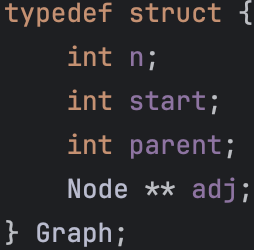
\includegraphics[]{img/graph.png}
\end{figure}
gdzie:
\begin{itemize}
    \item n - liczba wierzchołków grafu
    \item start oraz parent - zmienne potrzebne do podziału grafu
    \item adj - "lista" wierzchołków grafu
\end{itemize}

\newpage
\textbf{Struktura wierzchołka:}\\
\begin{figure}[ht]
  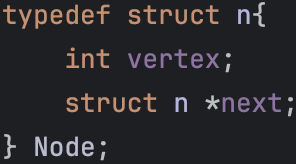
\includegraphics[]{img/node.png}
\end{figure}\\
gdzie:
\begin{itemize}
    \item vertex - etykieta wierzchołka
    \item next - wskaźnik do następnego wierzchołka
\end{itemize}


\section*{Funkcja podziału grafu}

\section*{Testy}
Przypadek testowy \textbf{make test1}:\\
Argumenty wywołania: \textbf{/testy/graf.csrrg 2 -t}\\\\
<prosta reprezentacja graficzne przypadku?>\\
<opis przypadku?>

\section*{Link do repozytorium:}
\url{https://github.com/t0q1/JIMP2_graph_C/tree/main}

\end{document}